\chapter{Обзор предметной области}
\label{chap:obzor}

    \section{Обозначения и сокращения} 
        \noindent\\
	    \textbf{RF} -- Radio Frequency \\
	    \textbf{RF-fingerprint} -- Radio Frequency Fingerprint \\
	    \textbf{MITM} -- Man In The Middle \\
	    \textbf{OFDM} -- Orthogonal Frequency-Division Multiplexing \\
	    \textbf{AE} -- Autoencoder\\
	    \textbf{RAW} -- Cырой, необработанный [сигнал]\\
        \textbf{ML} -- Machine Learning\\
	    \textbf{DT} -- Decision Tree\\
	    \textbf{TSNE (t-SNE)} -- t-distributed Stochastic Neighbor Embedding\\
	    \textbf{OSI} -- The Open Systems Interconnection model\\
	    \textbf{AGS} -- Automatic Gain Control\\
	    \textbf{DL} -- Deep Learning\\

    \newpage
    \section{Формальная запись проблемы}
        \par
            Сформулировать проблему можно так – необходимо с высокой точностью распознавать на физическом уровне устройства, сигнал которых мы уже принимали. \\
        \par
            Идентификация должна происходить вне зависимости от их конкретного расположения в пространстве, условий среды и зашумленности сигнала, а также с минимумом известных данных о конкретном устройстве. \\
        
        \par
            Ввиду своих физических свойств, – в случае OFDM, из-за преобразователей, усилителей и фильтров в схеме, – каждое передающее устройство уникально искажает сигнал. \\
            
            \begin{figure}[h!]
                \centering
                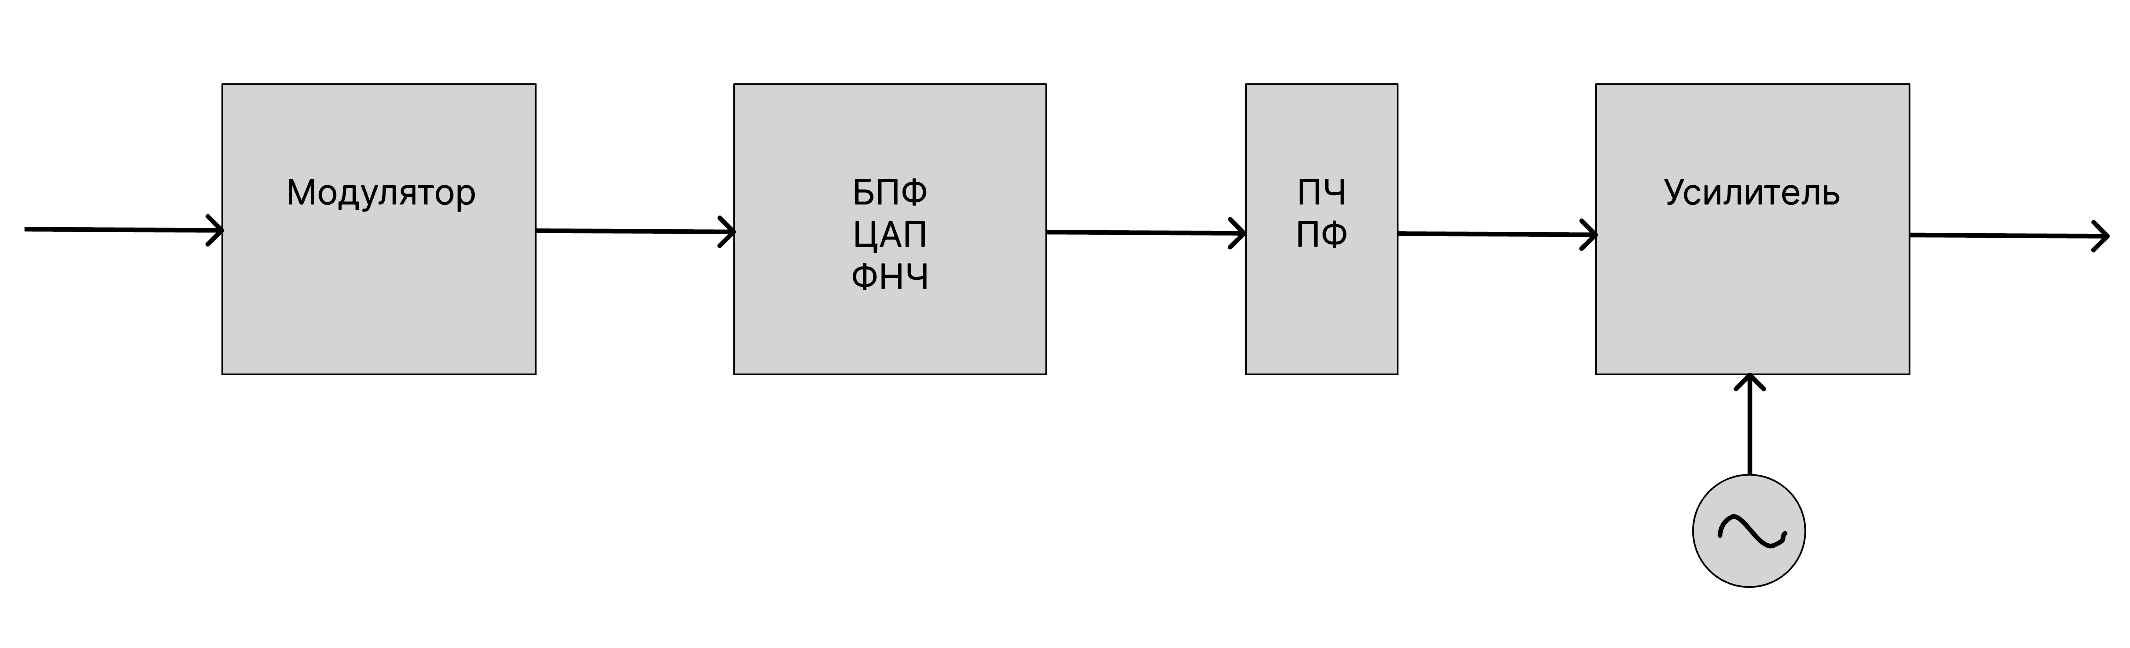
\includegraphics[scale=0.45]{pictures/index.png}
                \caption{Схема формирования OFDM-сигнала}
                \label{fig:my_label}
            \end{figure} 
            
        \par
            Для того, чтобы обнаружить внесенные искажения, необходимо выделить постоянные составляющие сигнала – преамбулы, после чего обработать их и решить задачу классификации на полученных данных.\\
            
            \begin{figure}[h!]
                \centering
                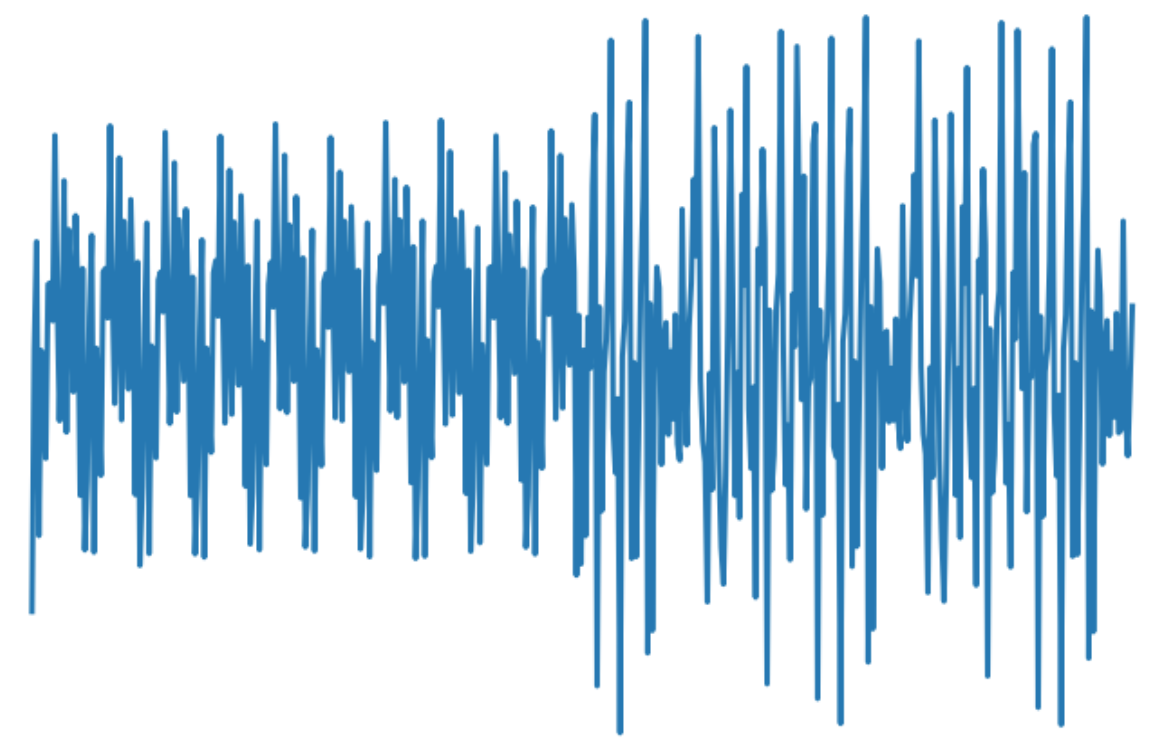
\includegraphics[scale=0.5]{pictures/preambules.png}
                \caption{Legacy преамбула}
                \label{fig:my_label}
            \end{figure} 
        \newpage
        \par
            В сигнале на Рис. 2 можно увидеть два поля legacy преамбулы: первая состоит из 10 одинаковых частей, а вторая из 2,5 одинаковых частей, с циклически расположенной начальной частью.
            \begin{figure}[h!]
                \centering
                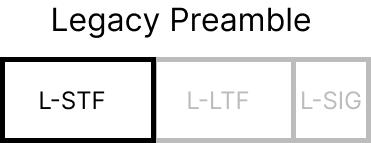
\includegraphics[scale=0.5]{pictures/L-STF.png}
                \caption{L-STF}
                \label{fig:my_label}
            \end{figure} 
        \par
            L-STF -- the Legacy short training field -- это первое поле 802.11 OFDM PLCP legacy преамбулы. \\
            \noindent
            Длительность L-STF зависит от полосы частот канала и составляет 8, 16 и 32 $\mu s$ для частот 20, 10 и 5 MHz соответственно.\\
            \noindent
            L-STF обладает хорошими корелляционными свойствами, поэтому используется для детекции начала пакетов, грубой частотной коррекции и установки AGC.\\
        \par
            \begin{figure}[h!]
                \centering
                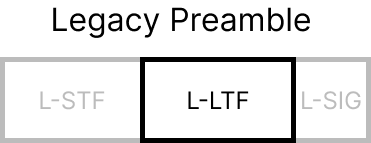
\includegraphics[scale=0.5]{pictures/L-LTF.png}
                \caption{L-LTF}
                \label{fig:my_label}
            \end{figure} 
            L-LTF -- the legacy long training field -- второе поле 802.11 OFDM PLCP legacy преамбулы.\\
            \noindent
            Длительность L-LTF также зависит от полосы частот канала и составляет 8, 16 и 32 $\mu s$ для частот 20, 10 и 5 MHz соответственно.\\
            \noindent
            L-LTF используется для оценки канала, точной оценки частотного смещения и точной оценки смещения символьной скорости.\\
        \newpage
            \begin{figure}[h!]
                \centering
                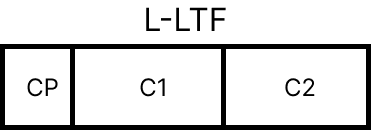
\includegraphics[scale=0.4]{pictures/L-LTF-1.png}
                \caption{Устройство L-LTF}
                \label{fig:my_label}
            \end{figure} 
        
        \par
            L-LTF состоит из циклического префикса (CP) и двух следующих друг за другом идентичных символов C1 и C2. CP имеет длительность в 2 раза меньшую, чем C1 и С2 и в точности повторяет вторую половину последнего во временной области. 
            
            
        
        \par
            При обработке сигнала для распознавания конкретного устройства в задаче радиометрической идентификации необходимо не только выделить особенности преамбул, но и избавиться от зашумленности сигнала, внесенной условиями среды. Именно поэтому при обработке RAW сигнала необходимо отобрать значимые для классификации признаки.
            
        \par
            
        
    \section{Постановка задачи}
    
        По RAW сигналам необходимо, пользуясь методами машинного обучения, решить задачу классификации -- распознавания каждого устройства, для которого ранее собиралась информация.
        
        
        
    
     



